\section{Indigo}
\authors{Kristina Heuser, Lena Trahe}

Der Farbstoff Indigo, der in einem intensiven dunkelblau/violett erscheint, kann aus der indischen Indigofera Pflanze, dem Färbewaid oder dem Färbeknöterich, wie bereits im Altertum, natürlich oder mit Hilfe der Heumann-Synthesen auf künstliche Weise gewonnen werden \cite{Schmidt,Steingruber}. Die erste Totalsynthese des Indigos aus Isatin, welches aus Phenylessigsäure dargestellt wurde, gelang 1878 dem Chemiker Adolf von Baeyer. In zwei weiteren wirtschaftlichen Syntheseverfahren wird Phenylglycin, welches aus Anilin, oder Phenylglycin-o-carbonsäure, welches aus Anthranilsäure hergestellt wird, mit Kaliumhydroxid zu Indoxyl verschmolzen (siehe Abb. \ref{fig:HeumannSynthese}). Indoxyl oxidiert weiter zu Indigo.

\begin{dsafigure}
 \centering
 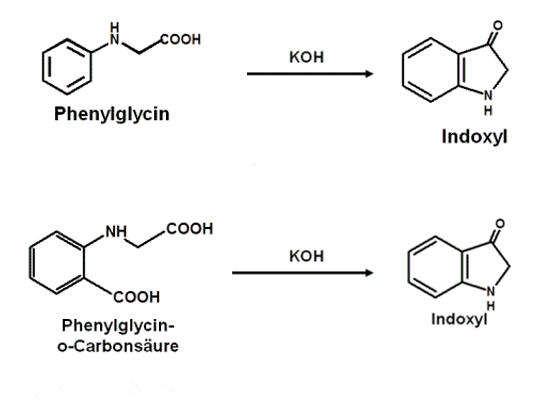
\includegraphics[width=\columnwidth]{HeumannSynthese.png}
 \caption{Heumann Synthesen des Indoxyls beziehungsweise Indigos \cite{HeumannSynthese}.}
 \label{fig:HeumannSynthese}
\end{dsafigure}

Der Farbstoff ist von wirtschaftlicher Bedeutung, da dieser in großen Mengen genutzt wird, um Textilien und Denim-Stoffe einzufärben. Dabei wird das zu verwebende Garn oder der Stoff in eine Leuko-Indigo-Lösung gegeben. Das Leuko-Indigo oxidiert an der Luft zum wasserunlöslichem, blauen Indigo (siehe Abb. \ref{fig:Reduktion}).

\begin{dsafigure}
 \centering
 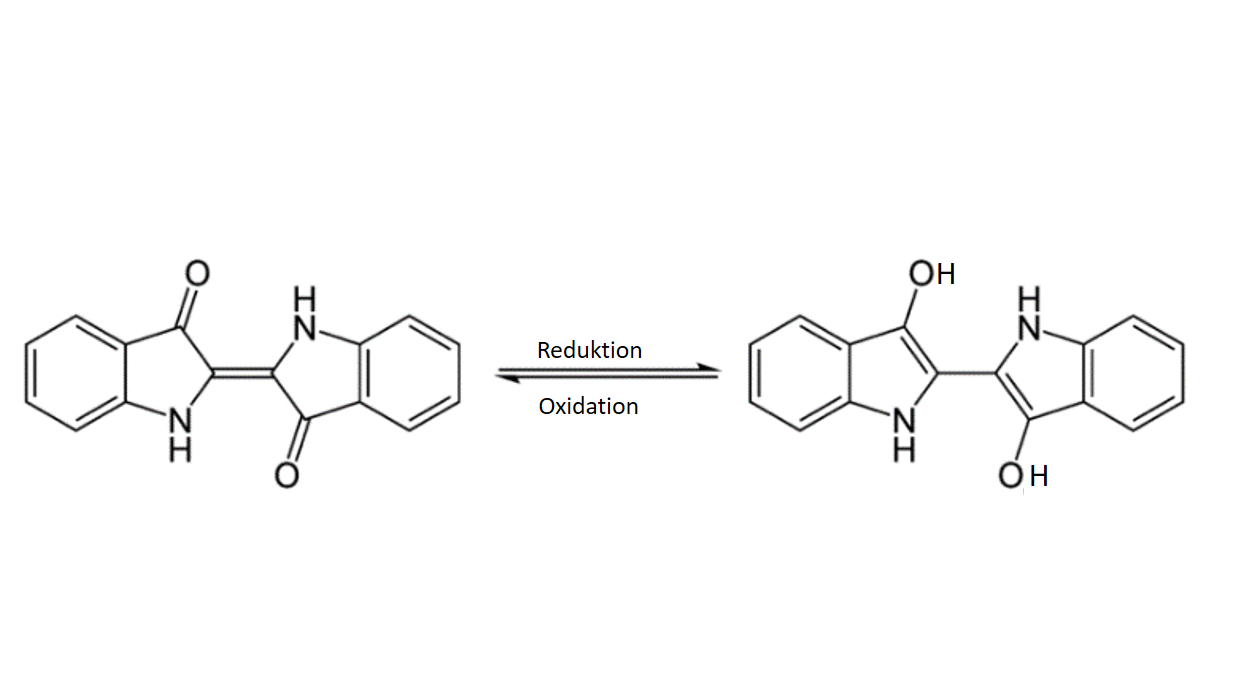
\includegraphics[width=\columnwidth]{Reduktion_Indigo.png}
 \caption{Reduktion des Indigos zu Leuko-Indigo und Oxidation des Leuko-Indigos zu Indigo \cite{Indigo_Reduktion}.}
 \label{fig:Reduktion}
\end{dsafigure}

Indigo hat die Summenformel $C_{16}H_{10}N_{2}O_{2}$ und besitzt zwei Carbonyl-Gruppen, welche durch die Reduktion protoniert und zu Hydroxyl-Gruppen werden.
Die Löslichkeit des Leuko-Indigos in Wasser lässt sich durch die entstandenen Hydroxyl-Gruppen erklären, da diese Wasserstoffbrückenbindungen eingehen können.
Der Wechsel der Farbe von gelb zu blau bei der Oxidation des Leuko-Indigos ist auf die Veränderung des $\pi$-Systems zurückzuführen.
 
